\section{}
\[
H(s)=\frac{-1+\j}{\sqrt{2}\,(s+1)^2}\,.
\]
\subsection{Bode-Diagramm}
\begin{center}
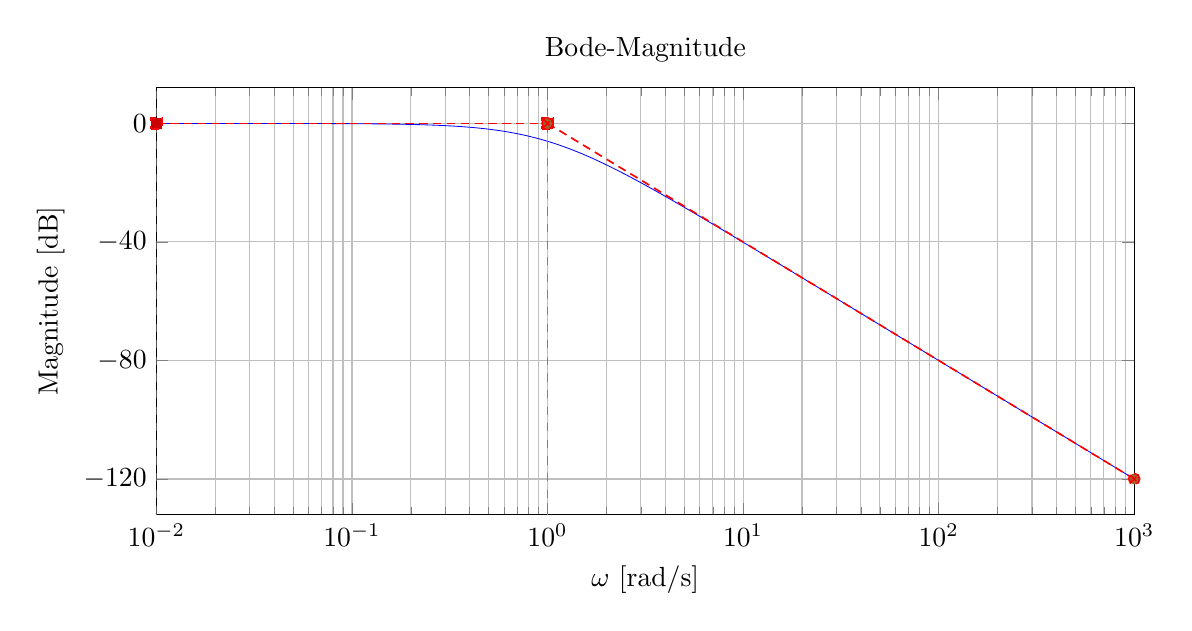
\begin{tikzpicture}
\begin{semilogxaxis}[
  width=14cm,height=7cm,
  xmin=1e-2,xmax=1e3,
  xlabel={$\omega$ [rad/s]},
  ylabel={Magnitude [dB]},
  grid=both,
  ytick distance=40,
  title={Bode-Magnitude}
]
\addplot[
  domain=1e-2:1e3,
  samples=600,
  mark=none,
  line width=0.3pt,
  blue
] {-40*ln(sqrt(1 + x^2))/ln(10)};
\addplot+[domain=1e-2:1,samples=2,dashed,dash pattern=on 3pt off 2pt,line width=0.6pt,red] {0};
\addplot+[domain=1:1e3,samples=2,dashed,dash pattern=on 3pt off 2pt,line width=0.6pt,red] {-40*ln(x)/ln(10)};
\draw[gray,dashed] (rel axis cs:0,0) -- (rel axis cs:0,1);
\draw[gray,dashed] (axis cs:1,\pgfkeysvalueof{/pgfplots/ymin}) -- (axis cs:1,\pgfkeysvalueof{/pgfplots/ymax});
\node[gray,anchor=south east] at (axis cs:1,\pgfkeysvalueof{/pgfplots/ymax}) {\scriptsize Pol $\omega_p=1$ (doppelt)};
\end{semilogxaxis}
\end{tikzpicture}
\vspace{6mm}
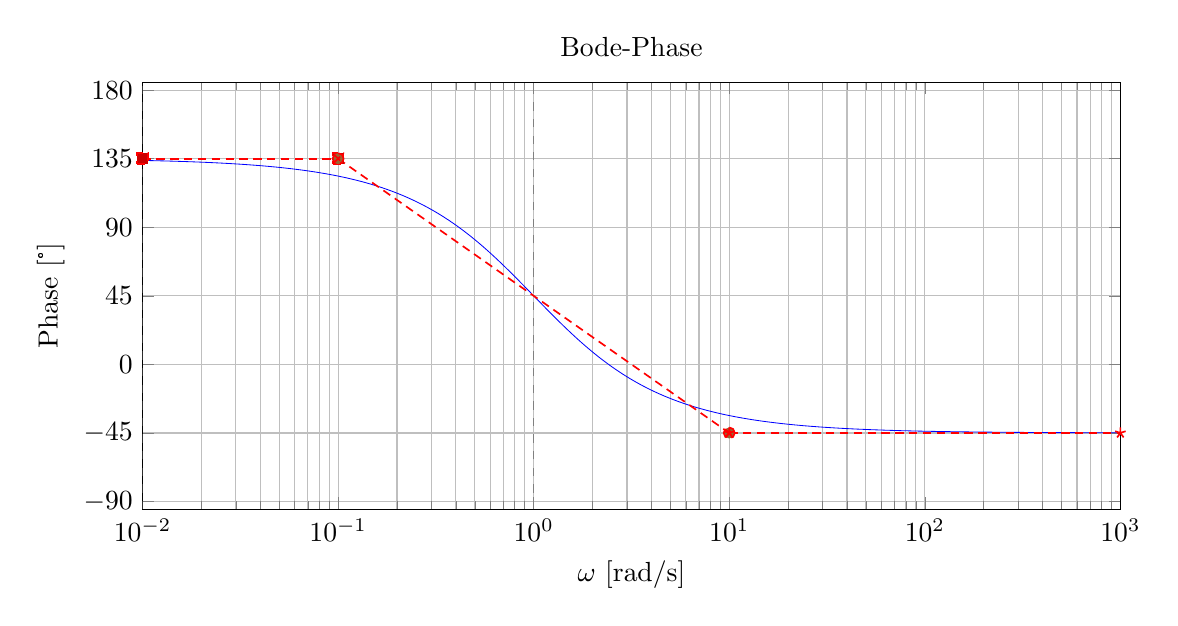
\begin{tikzpicture}
\begin{semilogxaxis}[
  width=14cm,height=7cm,
  xmin=1e-2,xmax=1e3,
  ymin=-95,ymax=185,
  ytick distance=45,
  xlabel={$\omega$ [rad/s]},
  ylabel={Phase [°]},
  grid=both,
  title={Bode-Phase}
]
\addplot[
  domain=1e-2:1e3,
  samples=600,
  mark=none,
  line width=0.3pt,
  blue
] {135 - 2*atan(x)};
\addplot+[domain=1e-2:1e-1,samples=2,dashed,dash pattern=on 3pt off 2pt,line width=0.6pt,red] {135};
\addplot+[domain=1e-1:1e1,samples=2,dashed,dash pattern=on 3pt off 2pt,line width=0.6pt,red] {45 - 90*ln(x)/ln(10)};
\addplot+[domain=1e1:1e3,samples=2,dashed,dash pattern=on 3pt off 2pt,line width=0.6pt,red] {-45};
\draw[gray,dashed] (rel axis cs:0,0) -- (rel axis cs:0,1);
\draw[gray,dashed] (axis cs:1,\pgfkeysvalueof{/pgfplots/ymin}) -- (axis cs:1,\pgfkeysvalueof{/pgfplots/ymax});
\node[gray,anchor=south east] at (axis cs:1,\pgfkeysvalueof{/pgfplots/ymax}) {\scriptsize Pol $\omega_p=1$ (doppelt)};
\end{semilogxaxis}
\end{tikzpicture}
\end{center}
\newpage

\subsection{Erklärung}
\begin{description}[leftmargin=1.2em,labelsep=.6em,font=\bfseries]

\item[1. Normalform herstellen.]
Bringe die Übertragungsfunktion in die Standardform.
\[
H(s)=\frac{K_0}{(1+sT_p)^2},\qquad
K_0=\frac{-1+\j}{\sqrt{2}}=\mathrm e^{\j 135^\circ},\quad T_p=1,\quad r=0.
\]
Zerlegung: \(\underline{F}_1(s)=\frac{1}{(1+sT_p)^2}\) (reelles Polglied zweiter Ordnung, doppelt); konstanter Phasor \(K_0\) mit \(|K_0|=1\), \(\arg K_0=+135^\circ\). Wir können $K_0$ behandeln als wäre es 1, aber müssen den gesamten Phasenplot um $135^\circ$ verschieben.

\item[2. Eckfrequenz bestimmen und sortieren.]
\[
\omega_p=\frac{1}{T_p}=1\,\mathrm{rad/s}.
\]
Nur diese Eckfrequenz; Sortierung trivial.

\item[3. Startpunkt des Amplitudengangs festlegen (Geradennäherung).]
\[
\omega_{\min}=\omega_p=1,\quad
F_{\mathrm{dB}}(\omega_{\min})=20\log_{10}\!\big(|K_0\underline{F}_{ges}^*(0)|\cdot \omega_{\min}^{\,r}\big)=0\,\mathrm{dB}.
\]
Anker für die Geradennäherung: \(0\,\mathrm{dB}\) bei \(\omega=1\).

\item[4. Verlauf links vom Startpunkt zeichnen.]
Für \(\omega<\omega_{min}\) bleibt die Amplituden-Asymptote bei \(0\,\mathrm{dB}\) konstant (Anfangssteigung \(r\cdot 20 \,\mathrm{dB}=0\)). Zeichne eine waagrechte Gerade links von der kleinsten Eckfrequenz.


\item[5. Steigungswechsel an der Eckfrequenz eintragen.]
Doppelpol: ab \(\omega=1\) Steigungsänderung um \(-40\,\mathrm{dB/dec}\).
Geradennäherung rechts:
\[
|H(j\omega)|_{\mathrm{dB}}\approx -40\log_{10}\omega\quad(\omega\ge 1).
\]

\item[6. Eckabrundung korrekt berücksichtigen.]
Bei \(\omega=\omega_p\) weicht der exakte Betrag um \(-6\,\mathrm{dB}\) von der Asymptote ab (Summe zweier \(-3\,\mathrm{dB}\), da Doppelpol):
\[
|H(j1)|_{\mathrm{dB}}=-20\log_{10}(1+1)=-20\log_{10}2\approx -6\,\mathrm{dB}.
\]

\item[7. Phasenstartwert festlegen.]
Konstanter Phasor \(K_0\) liefert einen Offset \(+135^\circ\).
Für \(\omega\to 0\): \(\varphi(0)=+135^\circ\).

\item[8. Phasenänderung durch das Polglied eintragen.]
Ein Doppelpol bewirkt insgesamt \(-180^\circ\) über die Dekade \([0.1,10]\) (je \(-90^\circ\) pro einfachem Pol). Näherung:
\[
\varphi(\omega)\approx
\begin{cases}
+135^\circ,& \omega\le 0.1,\\
45^\circ-90^\circ\log_{10}\omega,& 0.1<\omega<10,\\
-45^\circ,& \omega\ge 10.
\end{cases}
\]

\item[9. Grenzwerte und Konsistenz prüfen.]
DC: \(|H(0)|=|K_0|=1\Rightarrow 0\,\mathrm{dB}\), \(\varphi(0)=+135^\circ\).
HF: \(|H(j\omega)|\sim 1/\omega^{2}\Rightarrow -40\log_{10}\omega\,\mathrm{dB}\), \(\varphi(\infty)=+135^\circ-180^\circ=-45^\circ\).
Pol-/Nullzählung: \(m=0\), \(n=2\Rightarrow (m-n)\cdot 90^\circ=-180^\circ\) plus Offset \(+135^\circ\) durch \(K_0\) ergibt \(-45^\circ\).

\end{description}

\subsubsection*{Stückweise Näherungen (für die Skizze)}
\[
|H(j\omega)|_{\mathrm{dB}}\approx
\begin{cases}
0,& \omega\ll 1,\\[2pt]
-20\log_{10}2,& \omega=1,\\[2pt]
-40\log_{10}\omega,& \omega\gg 1,
\end{cases}
\]\[
\varphi(\omega)\approx
\begin{cases}
+135^\circ,& \omega\le 0.1,\\[2pt]
45^\circ-90^\circ\log_{10}\omega,& 0.1<\omega<10,\\[2pt]
-45^\circ,& \omega\ge 10.
\end{cases}
\]

\newpage